\documentclass[
10pt, % Main document font size
letterpaper, % Paper type, use 'letterpaper' for US Letter paper
oneside, % One page layout (no page indentation)
%twoside, % Two page layout (page indentation for binding and different headers)
headinclude,footinclude, % Extra spacing for the header and footer
BCOR5mm, % Binding correction
]{scrartcl}


\usepackage{mike}
% include image package and the images folder
\graphicspath{ {Diagrams/} }

%----------------------------------------------------------------------------------------
%	TITLE AND AUTHOR(S)
%----------------------------------------------------------------------------------------

\title{\normalfont\spacedallcaps{Remote EJB Setup and Invocation}} % The article title

\author{\spacedlowsmallcaps{Michael Meding* , mikeymeding@gmail.com}} % The article author(s) - author affiliations need to be specified in the AUTHOR AFFILIATIONS block

\date{} % An optional date to appear under the author(s)

%----------------------------------------------------------------------------------------

\begin{document}

\maketitle % Print the title and abstract box

\setcounter{tocdepth}{2} % Set the depth of the table of contents to show sections and subsections only

\tableofcontents % Print the contents section

\thispagestyle{empty} % Removes page numbering from the first page

%----------------------------------------------------------------------------------------
%	ARTICLE CONTENTS
%----------------------------------------------------------------------------------------
 
\section*{Abstract}
This article details a ground up intro to setting up a remote EJB and invoking a method from it. This involves setting up your application server which for this article I used Wildfly. Wildfly is a popular and highly portable application server that is well suited for this task. Unfortunately setting up a remote EJB on wildfly requires many specific settings so this setup does not apply to other application servers. For this article I assume that the reader has a good foundation in Java and understands RESTful web architecture, Additionally I assume that the reader has a fair understanding of how enterprise applications work using Java EE 7.
 
~\newline

\begin{figure}[h]
\centering
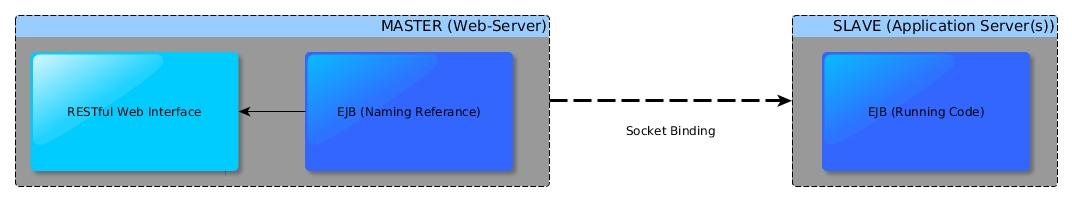
\includegraphics[width=15.5cm]{EJBDiagram} % FLOWCHART
\caption{A typical remote EJB setup using 2 servers (Master and Slave)}
\label{fig:servers}
\end{figure}

\paragraph{Before We Begin} First off, what the hell is an EJB anyway and why do I need it? EJB stands for Enterprise Java Bean and it is a wonderful container that packages your code into neat little blocks that can be deployed anywhere. If you are familiar with enterprise coding, or even coding a large project, then you know how important scalability of your code can be.  EJB's allow you to have the ultimate in scalability while still retaining or perhaps improving execution speed. EJB's get packaged into .jar/.ear files just like standard Java but are then deployed using an application server, like Wildfly, to allow them to be called upon remotely.

%------------------------------------------------

\section{Setting Up Wildfly standalone-full.xml}

%------------------------------------------------

\paragraph{} The following 3 subsections of this document cover how to set up your standalone-full.xml file. This is the main configuration file for wildfly. If you do not already have a working local wildfly setup then you should begin by going through the tutorial pages \href{https://docs.jboss.org/author/display/WFLY8/Getting+Started+Developing+Applications+Guide}{here.}

%------------------------------------------------

\subsection{secret}

%------------------------------------------------

\paragraph{XML}~
%Code Snippet
\lstsetxml % bring in xml highlight settings
\begin{lstlisting}[language=XML]
<security-realm name="ejb-security-realm">
	<server-identities>
		<secret value="Y2NhZXMx"/>
	</server-identities>
</security-realm>
\end{lstlisting}

\paragraph{} To start off you need to add a security-realm at the top of your standalone-full.xml just after the extensions. Please note that throughout the standalone file the names of some items will match others. This is necessary for wildfly to determine links between the different objects. 

%------------------------------------------------

\subsection{remote-mallorca}

%------------------------------------------------

\paragraph{XML}~
%Code Snippet
\lstsetxml % bring in xml highlight settings
\begin{lstlisting}[language=XML]
<--! FROM THIS -->
<subsystem xmlns="urn:jboss:domain:remoting:2.0">
	<endpoint worker="default"/>
	<http-connector name="http-remoting-connector" connector-ref="default" security-realm="ApplicationRealm"/>
</subsystem>

<--! TO THIS -->
<subsystem xmlns="urn:jboss:domain:remoting:2.0">
	<endpoint worker="default"/>
	<http-connector name="http-remoting-connector" connector-ref="default" security-realm="ApplicationRealm"/>
	<outbound-connections>
		<remote-outbound-connection name="remote-mallorca-connection" outbound-socket-binding-ref="remote-mallorca" username="uwe" security-realm="ejb-security-realm" protocol="http-remoting">
			<properties>
				<property name="SASL_POLICY_NOANONYMOUS" value="false"/>
				<property name="SSL_ENABLED" value="false"/>
			</properties>
		</remote-outbound-connection>
	</outbound-connections>
</subsystem>
\end{lstlisting}


\paragraph{} In the base standalone file there exists a subsystem with the remoting:2.0 keyword. Initially it only has one default endpoint which is the default ApplicationRealm. You need to add a section called outbound-connections which contains all the information about your connection. The security-realm name must match the one we described in the section above, additionally the names that you specify in this section will be reused elsewhere so make a habit of knowing which one is which. I used the name mallorca for my setup as the server which will be hosting my code is called mallorca.

%------------------------------------------------

\subsection{outbound-socket-binding}

%------------------------------------------------

\paragraph{XML}~
%Code Snippet
\lstsetxml % bring in xml highlight settings
\begin{lstlisting}[language=XML]
<outbound-socket-binding name="remote-mallorca">
	<remote-destination host="10.0.0.154" port="8080"/>
</outbound-socket-binding>
\end{lstlisting}

\paragraph{} Lastly, at the bottom of the file there is a section called socket-binding-group. In this section you need to describe the physical address of the server that will be hosting your remote EJB. The name must match that described by outbound-socket-binding-ref defined in the section above. Typically the port for this will be 8080 but if there is more than one .jar file deployed at this address it will have different port number. Keep in mind that you will be deploying your server-side code to localhost of the host server. This means that you will have to set up some routing on the server side but we will get to that later.


%------------------------------------------------

\section{Master's Side Application Code}

%------------------------------------------------

\paragraph{} This code is all contained in the RESTful web side as described in Figure~\ref{fig:servers}. For this application I used a REST interface to call my remote method. To call my REST interface I simply used a line in curl such as "curl -v -X POST http://localhost:8080/project-name/blahblahmethod".

%------------------------------------------------

\subsection{@EJB}

%------------------------------------------------

\paragraph{JAVA EE}~
%Code Snippet
\lstsetjava % brings in the java code highlight parameters
\begin{lstlisting}[language=Java]
@EJB
Distribution dist;
\end{lstlisting}

\paragraph{} This tells us that we have an EJB and it is described by the Distribution class. However, this does not resolve where the code actually exists only that we have one.

%------------------------------------------------

\subsection{@PostConstruct}

%------------------------------------------------

\paragraph{JAVA}~
%Code Snippet
\lstsetjava % brings in the java code highlight parameters
\begin{lstlisting}[language=Java]
@PostConstruct
private void init() {
	try {
		Properties props = new Properties();
		props.put(javax.naming.Context.URL_PKG_PREFIXES, "org.jboss.ejb.client.naming");
		javax.naming.Context context = new javax.naming.InitialContext(props);		
		dist = (Distribution) context.lookup("ejb:/acq-distribution-ejb-1.0/DistributionImpl!os.oss.Distribution");
	} catch (Exception e) {
		log.severe(e.getMessage());
	}
}
\end{lstlisting}

\paragraph{} @PostConstruct applies the url properties and performs a remote EJB lookup. If the class is found it is executed on the remote. If the class is not found it is executed on the local machine and a message will be logged detailing the reason for a bad connection. As you can see the naming pattern for the .lookup is quite specific and follows a syntax as such,
\begin{description}
\item[For stateless beans.] \hfill \\
\textbf{
ejb:<app-name>/<module-name>/<distinct-name>/<bean-name>!<fully-qualified-classname-of-the-remote-interface>}
\item[For stateful beans.] \hfill \\
\textbf{
ejb:<app-name>/<module-name>/<distinct-name>/<bean-name>!<fully-qualified-classname-of-the-remote-interface>?stateful}
\item[app-name :] \hfill \\
This is the name of the .ear (without the .ear suffix) that you have deployed on the server and contains your EJBs.
\item[module-name :] \hfill \\
This is the name of the .jar (without the .jar suffix) that you have deployed on the server and the contains your EJBs. If the EJBs are deployed in a .war then the module name is the .war name (without the .war suffix).
\item[distinct-name :] \hfill \\
This is a WildFly-specific name which can be optionally assigned to the deployments that are deployed on the server. More about the purpose and usage of this will be explained in a separate chapter. If a deployment doesn't use distinct-name then, use an empty string in the JNDI name, for distinct-name
\item[bean-name :] \hfill \\
This is the name of the bean for which you are doing the lookup. The bean name is typically the unqualified classname of the bean implementation class, but can be overriden through either ejb-jar.xml or via annotations. The bean name part cannot be an empty string in the JNDI name.
\item[fully-qualified-classname-of-the-remote-interface :] \hfill \\
This is the fully qualified class name of the interface for which you are doing the lookup. The interface should be one of the remote interfaces exposed by the bean on the server. The fully qualified class name part cannot be an empty string in the JNDI name.
\end{description}

\paragraph{\textbf{NOTE:}} One useful way to find the lookup name of an EJB is to look at the wildfly logs upon startup. There will be a block that describes all discovered \textbf{LOCAL} EJB's. To get the remote equivalent you need to change the java: prefix to ejb: so long as you have the same deployment on both your local and remote. Also note that if you have your EJB's deployed inside of an EAR (Enterprise Archive) then you must append the name of the ear before the name of your EJB in the lookup string. The syntax for a remote call inside of an ear would then roughly follow the pattern: \textbf{ejb:<ear-name>/<ejb-name>/<class-syntax(as above)>}.

%------------------------------------------------

\subsection{jboss-ejb-client.xml}

%------------------------------------------------

\paragraph{XML}~
%Code Snippet
\lstsetxml % bring in xml highlight settings
\begin{lstlisting}[language=XML]
<jboss-ejb-client xmlns="urn:jboss:ejb-client:1.0">
	<client-context>
		<ejb-receivers>
			<remoting-ejb-receiver outbound-connection-ref="remote-mallorca-connection"/>
		</ejb-receivers>
	</client-context>
</jboss-ejb-client>
\end{lstlisting}

\paragraph{} For this example we are trying to avoid tedious .properties files describing our endpoints. This becomes difficult to maintain especially when you move a bunch of EJB's to a new server. So for this reason we just tell our web application that we might have some EJB's at the location described by remote-mallorca-connection in our standalone. This file belongs in the WEB-INF folder of your web project.


%------------------------------------------------

\section{Slave Side Code Deployment}

%------------------------------------------------

%------------------------------------------------

\subsection{standalone-full.xml}

%------------------------------------------------

\paragraph{XML}~
%Code Snippet
\lstsetxml % bring in xml highlight settings
\begin{lstlisting}[language=XML]
<interfaces>
        <interface name="management">
            <inet-address value="${jboss.bind.address.management:0.0.0.0}"/>
        </interface>
        <interface name="public">
            <inet-address value="${jboss.bind.address:0.0.0.0}"/>
        </interface>
        <interface name="unsecure">
            <inet-address value="${jboss.bind.address.unsecure:0.0.0.0}"/>
        </interface>
</interfaces>
\end{lstlisting}
 
\paragraph{} The only modification that you need to make to the standalone.xml file from a base setup is to change all occurrences of the localhost bind address (127.0.0.1) to (0.0.0.0). This is great because it makes it super easy to deploy code on new servers.

%------------------------------------------------

\subsection{Please Note!}

%------------------------------------------------

% explain here about needing a correct user to gain access to EJB
\paragraph{} The last thing that must be done on the slave server is to add a user. Wildfly is set up to have 2 different types of users, Management Users and Application Users. If you wish to access the Wildfly web console then you must have a Management User set up as your login. If you wish to access EJB's then you must have a Application User that matches the user information that we put into the standalone-full.xml on the master size. If no Application User exists then you will receive an unauthorized exception in your log file only, and perhaps a null pointer in your code. To set up a new Wildfly user you must execute the add-user script in the bin folder of your Wildfly server and follow the instructions creating an Application User with no group info.


\end{document}
